\documentclass{article} % article doctype, possible font size range from 8pt to 20pt with not all being avaiable.
\title{\huge Willy The Robot Hardware Design}
\author{Jeroen van 't Hul\\S1139163  \and Thomas Zwaanswijk\\s1089273 \and Tom van den Noort\\s1101124}
\date{\parbox{\linewidth}{\centering%
	\today\endgraf\bigskip
	Supervisor \hspace*{3cm} Main Stakeholder \endgraf\medskip
	Mischa Mol \hspace*{3cm} Ilja Clabbers \endgraf\bigskip
	Windesheim Zwolle\endgraf}} 


% include packages
\usepackage{graphicx}
\usepackage{caption}
\usepackage{mathabx}
\usepackage{wrapfig}
\usepackage[margin=1.0in]{geometry} % sets page margin, 2.0in is default.
\usepackage{titlesec}
\usepackage{hyperref}
\usepackage[table,xcdraw]{xcolor}
\usepackage{float}
\usepackage[export]{adjustbox}
\usepackage{todonotes}
\usepackage{indentfirst}
\usepackage{blindtext}
\usepackage{scrextend}
\usepackage{apacite}
%\usepackage{siunitx}
%\usepackage{multirow}	% used for table multirow support
%\usepackage{longtable} % Allows tables to roll over into a new page.
\usepackage[nottoc,numbib]{tocbibind} % Adds bibliography / references to TOC and numbers that section.
\usepackage{array}
\usepackage{footnote}

% ----- custom commands ----- %
% Wrapper for paragraph command. Forces newline after paragraph title
\newcommand{\myparagraph}[1]{\paragraph{#1}\mbox{}\\} % Without \mbox{} all newlines will be ignored, making the first sentence appear on the same line as a paragraph title.
% monospace codeblock
\def\code#1{\texttt{#1}}
% changing the ToC depth in the document enviroment
\newcommand{\changelocaltocdepth}[1]{%
	\addtocontents{toc}{\protect\setcounter{tocdepth}{#1}}%
	\setcounter{tocdepth}{#1}%
}

\restylefloat{table}

\newcolumntype{L}[1]{>{\raggedright\let\newline\\\arraybackslash\hspace{0pt}}m{#1}}
\newcolumntype{C}[1]{>{\centering\let\newline\\\arraybackslash\hspace{0pt}}m{#1}}
\newcolumntype{R}[1]{>{\raggedleft\let\newline\\\arraybackslash\hspace{0pt}}m{#1}}

\makesavenoteenv{tabular}
\makesavenoteenv{table}

\setcounter{tocdepth}{2} % only part,chapters,sections, subsections appear in ToC

\addtokomafont{labelinglabel}{\sffamily}

\DeclareCaptionFormat{cancaption}{#1#2#3\par} % Normal format actually
\DeclareCaptionLabelFormat{cancaptionlabel}{#1}
\captionsetup[figure][number]{format=cancaption,labelformat=cancaptionlabel}
\graphicspath { {images/}{../images/} }

\begin{document}
\maketitle

\begin{figure}[H]
\centering
\includegraphics[width=12 cm]{WTRLogo.png}
\end{figure}
\thispagestyle{empty}
\newpage
\setcounter{page}{1}
\tableofcontents
\newpage

% Sections
\section{Batteries and Wiring}
Towards the end of the project a small fire caused by contact between the power-jack of the TV and a car battery meant that one of the transformers partially melted.
This spurred the group to redo the electronic set-up of WTR.
Those changes are documented here.

\subsection{Removal of 2 batteries}
The batteries used are lead-based batteries, capable of delivering 12 volts each.
They are set up in two group of two, so that there are two sets parallel.
This outputs a total of $24V$, which is more than most equipment used operates on.
As such, several transformers are used.
These are located in a small black box with white fan cover on it.
There are 3 transformers used, each of which outputs one of the following voltages:
\begin{itemize}
\item $5V$ - Powers the 4 raspberry Pi's
\item $9V$ - Powers the switch connecting all the Ethernet cables
\item $19V$ - Powers the TV screen as well as the LDIAR
\end{itemize}

There used to be a $12V$ voltage converter, but since the fire incident took place at the end of the time allotted to this group, simply changing the voltage the LIDAR operates at seemed more prudent than waiting for a new converter.
As such, the TV and the LIDAR now share a power source.
The safe operating voltage of the LIDAR can lie anywhere between $9-28V$, so $19V$ is perfectly safe.


\subsection{Wiring}
Due to the aforementioned fire incident, a new power switch was installed as well.
Instead of 4 separate switches for each voltage level, instead a single master switch is used, as is shown in fig \ref{fig::wiringschem}

\begin{figure}
\centering
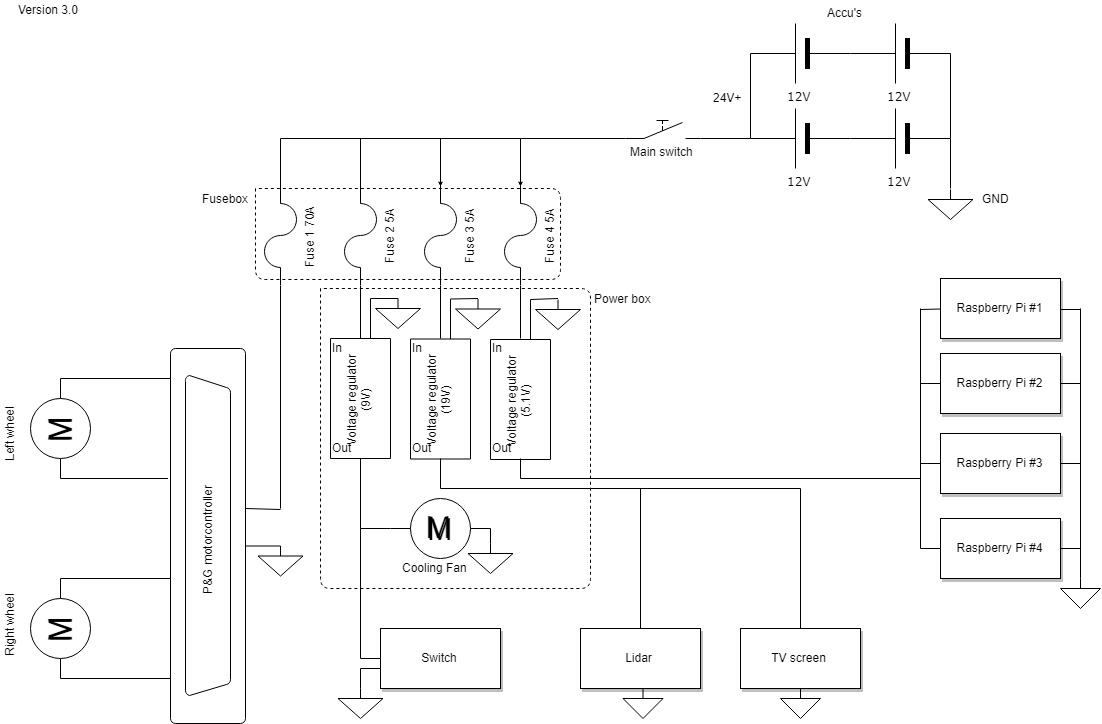
\includegraphics[width=16cm]{wiringSchem.PNG}
\caption{Schematic showing the wiring set-up of WTR}
\label{fig::wiringschem}
\end{figure}

This change was implemented because it allows a quick disengagement of the motors, rather than killing the motor controller.


\subsubsection{Fuses}
Currently, WTR uses 3 $5A$ universal car fuses, which should prevent any of the devices being overloaded.
In case this is not enough, several other fuses ranging from $5A$ to $30A$ can be found in cupboard C in the innovation lab on T5.
The electric motors are secured with a $70A$ fuse, should this not be enough a new fuse will need to be obtained, as there were no spares.
\newpage

\section{IMU}
The IMU \ref{trm::imu} that was present on WTR before, the MPU6050, was broken when the current group started work on the project.
As such, a replacement had to be chosen.
Rather than go with a 6-axis IMU such as the MPU6050, a 9-axis IMU seemed the better option, so an analysis was done to determine the best device.

The demands were as follows:
\begin{enumerate}
\item Device must have an accelerometer, gyroscope and magnetometer
\item Device must be Arduino/Pi compatible
\item Device must be affordable within the budget given by the product owner
\item Device must be accurate enough to contribute to the solution
\end{enumerate}

The following devices were selected as potentially viable options:
\begin{enumerate}
\item \href{https://www.sparkfun.com/products/13762}{MPU9250}- Sparkfun breakout
\item \href{https://store.arduino.cc/9-axis-motion-shield}{BNO055} - Arduino motionshield
\item \href{https://learn.adafruit.com/nxp-precision-9dof-breakout/overview}{NXP} - Adafruit breakout
\end{enumerate}

Each device has its features outlined in the following table:

\begin{figure}[H]
    \begin{tabular}{|c|c|c|c|c|c|}
    \hline
    \textbf{device} & \textbf{cost} & \textbf{operating voltage $V$} & \textbf{angular scale $^O /sec$} & \textbf{acceleration scale $G$}  & \textbf{format} \\ \hline
    MPU9250 & \$ 14,95 & 2.4 - 3.6 & 250 - 2000 & 2 - 16 & breakout board \\ \hline
    BNO055  & \$ 23,95 & 2.4 - 3.6 & 250 - 2000 & 2 - 16 & Arduino Shield \\ \hline
    NXP     & \$ 14,95 & 2 - 3.6   & 250 - 2000 & 2 - 8   & breakout board \\ \hline
    \end{tabular}
\caption{comparison of features of the three selected 9-axis IMU's}
\label{tbl::IMUcomp}
\end{figure}

The three sensors here are fairly similar, though there are a few critical differences.
The MPU9250 and the NXP are very similar, and even have the same price.
Out of those 2, the MPU has a slightly higher range in the acceleration scale category, which for no added price, meaning it knocks out the NXP.
The MPU9250 and the BNO055 have the same sensitivity, but the price of the BNO055 is significantly higher than the MPU9250.
Therefore, the logical conclusion is that the MPU9250 should be used.

Figures were obtained from the following places:
\begin{itemize}
\item MPU9250 - \cite{mpu}
\item BNO055  - \cite{bno}
\item NXP - \cite{nxp1} , \cite{nxp2}
\end{itemize}


\subsection{Hardware Setup}
The wiring for the MPU9250 is as follows:

\begin{figure}[H]
\centering
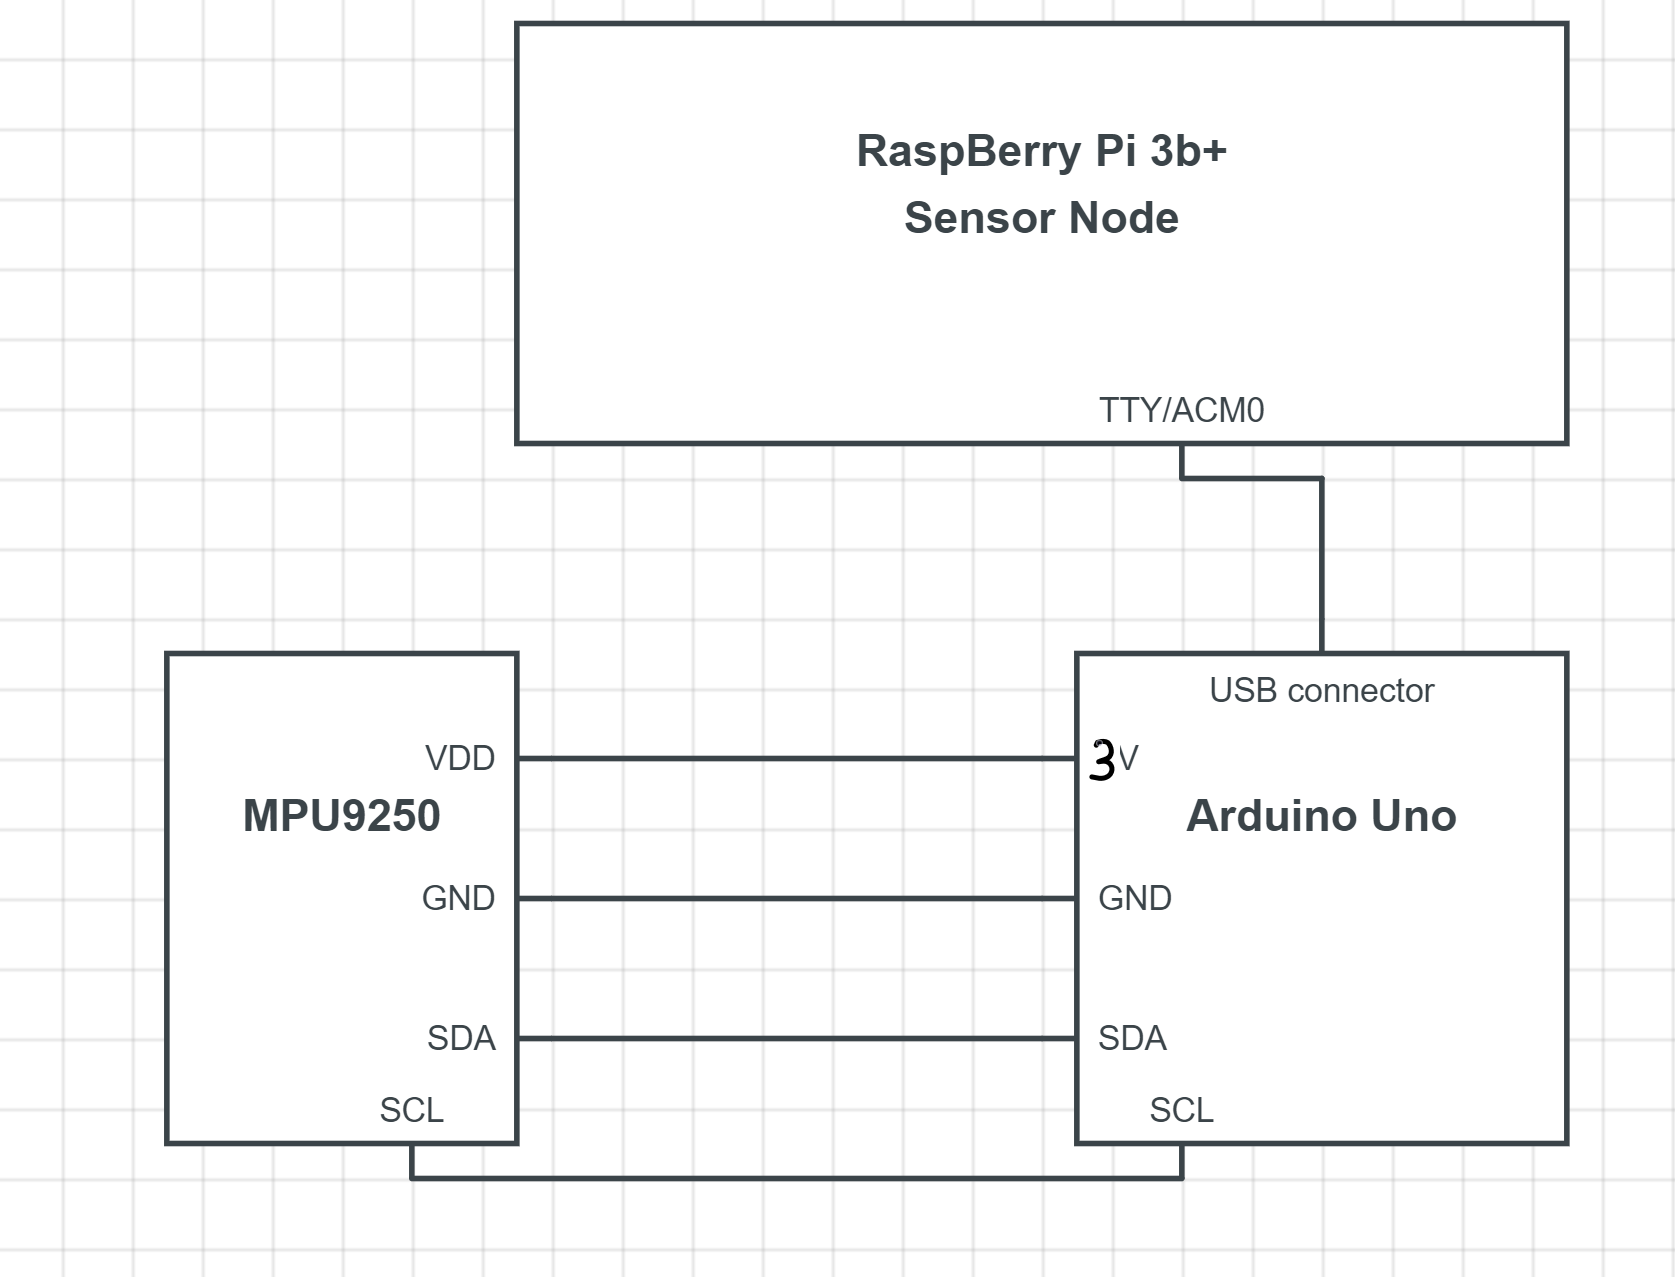
\includegraphics[width=12cm]{wires.png}
\caption{Wiring setup for the MPU to Arduino communication}
\label{fig::wiring}
\end{figure}

The pins used on the arduino are as follows: 
\begin{figure}[H]
\centering
\begin{tabular}{|c|c|}
\hline
\textbf{Pin} & \textbf{Function} \\ \hline
Analogue 4 & SDA     \\ \hline
Analogue 5 & SCL     \\ \hline
GND        & ground  \\ \hline
3.3V       & VDD     \\ \hline
\end{tabular}
\end{figure}

\subsubsection{Address}
In the example code it is stated the the address of the MPU9250 should be \code{0x71}.
This is not the case, and instead the address is \code{0x73}.
The reason for this difference is not clear, but it does not pose a problem other than the code used not matching the examples.
The magnetometer, the AK8963, has the same address as mentioned in documentation about it, as well as the example code.

\subsubsection{Positioning}
During the development, a problem came up.
A magnetometer is reliant on, as the name implies, magnetism.
Since the frame is made of steel, it interferes with the magnetometer.
When the IMU is mounted to the frame, the quaternion it outputs is essentially always the same, since the magnetic values never change.
If the robot turns, the magnetic field it produces turns with it.
This is known as "soft iron interference".

To combat this issue, there are two solutions.
The first would be to somehow isolate the frame, electric motors and car batteries so that the magnetic field is contained.
No one in the current group has the expertise or knowledge to do this, and it would probably also weigh down WTR so much the robot would become nearly immovable.
The second option is to move the sensor as far away from the source of the interference as possible.
To this end, a case has been designed which can be hung from the top of the screen, as far away from the magnetic influences of the robot as possible.

\newpage    
    
\section{SONARS}
The sonar sensors where already present on WTR, but the implemention lacks professionality and long term stability was at risk, both at mechanical, eletrical and software level.
The improvements are described in each of these aspects in the folling sections.

\subsection{Mechanical setup}
Instead of zipties and tape a special clamp, ball joint and housing for the HC-SR04 was designed in solidworks and 3D printed. See figure below.
There are eight sensors which are stategically placed around WTR.
The clamp (orange) is desgined to fit around the 25mm sqaure tubes which are present around WTR. 
This clamp is provided with an opening which will hold the ball clamp (red).
The ball (green) can be pressed in the ball clamp easily and will create a ball joint mechanism.
Ball is provided with a tapered shaft which is pressed into the housing (blue).
The housing holds the sonar senor, and is closed with a lid (grey).

\begin{figure}[H]
\centering
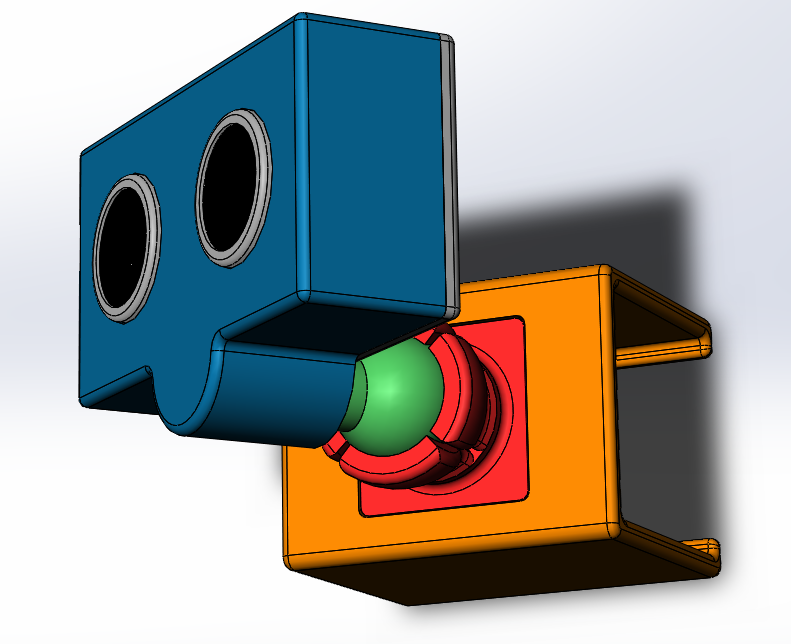
\includegraphics[width=12cm]{SonarSensorAssembly.png}
\caption{Sonar sensor assembly}
\label{fig::sonarassembly}
\end{figure}


\subsection{Electrical setup}
Instead of breadbord and a lot of lose wires a special wiring harnass was designed. 
This harnass is split into two sections, one for the three front sensors and one for the five back sensors.
The sections meet in the middle and connect to the arduino Uno.
The sections contain the common power wires, the common trigger wire and indivdual echo wires.
The wires are made from flat cable and provided with connectors which improves repair or reorientation if needed.

The wiring for the sonars can be found in the schematic below:

\begin{figure}[H]
\centering
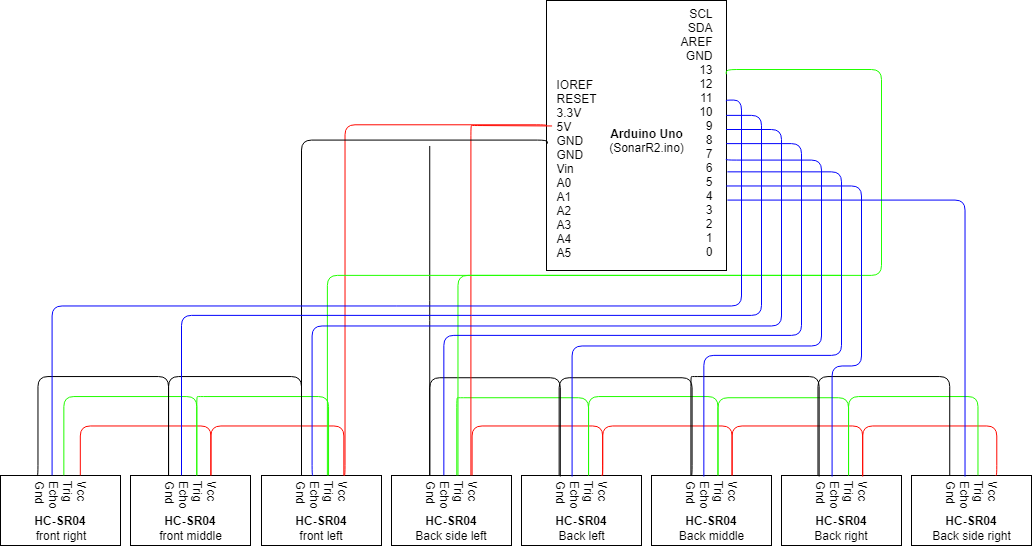
\includegraphics[width=12cm]{SonarDiagram.png}
\caption{Wiring setup for the 8 sonar sensors to Arduino communication}
\label{fig::wiringsonar}
\end{figure}

 
    
\section{Motor Controller}
The motor controller consists of two parts.
The first is the Arduino Mega 2560, located in a black box underneath the laptop, on top of the batteries.
The second are two rotary encoders \cite{roten}, located on the two front wheels.
These are wired to the arduino via 2 gray ribbon cables.

\subsection{Arduino Mega 2560}
This was already a part of the solution before the 2019 Q1 \& Q2 group started work on the project.
Using the pre-existing connections made by previous groups where old rotary encoders were attached, the new rotary encoders have been connected.

\subsection{Rotary Encoders}
These rotary encoders were chosen based on the following criteria:

\begin{itemize}
\item Encoders must have a resolution of at least 1024 PPR \ref{trm::PPR}
\item Encoders must run of a 3.3 or 5V current
\item Encoders must be attachable to the wheels, either through pre-fabricated attachments or 3d-printable sockets
\item Encoders must be priced within the budget provided by the product owner
\item Encoders must be able to record both directions
\end{itemize}

The Bourns encoders chosen satisfy all the given criteria.
While the documentation states that there are 256 cycles per revolution, each cycle produces 4 pulses.
This adds up to 1024 Pulses Per Revolution.


\subsubsection{Flexible Coupling}
The rotary encoders have been socketed on the axles using a 3-d printed mount, using the coupling shown in fig \ref{fig::FCR}.

\begin{figure}[H]
\centering
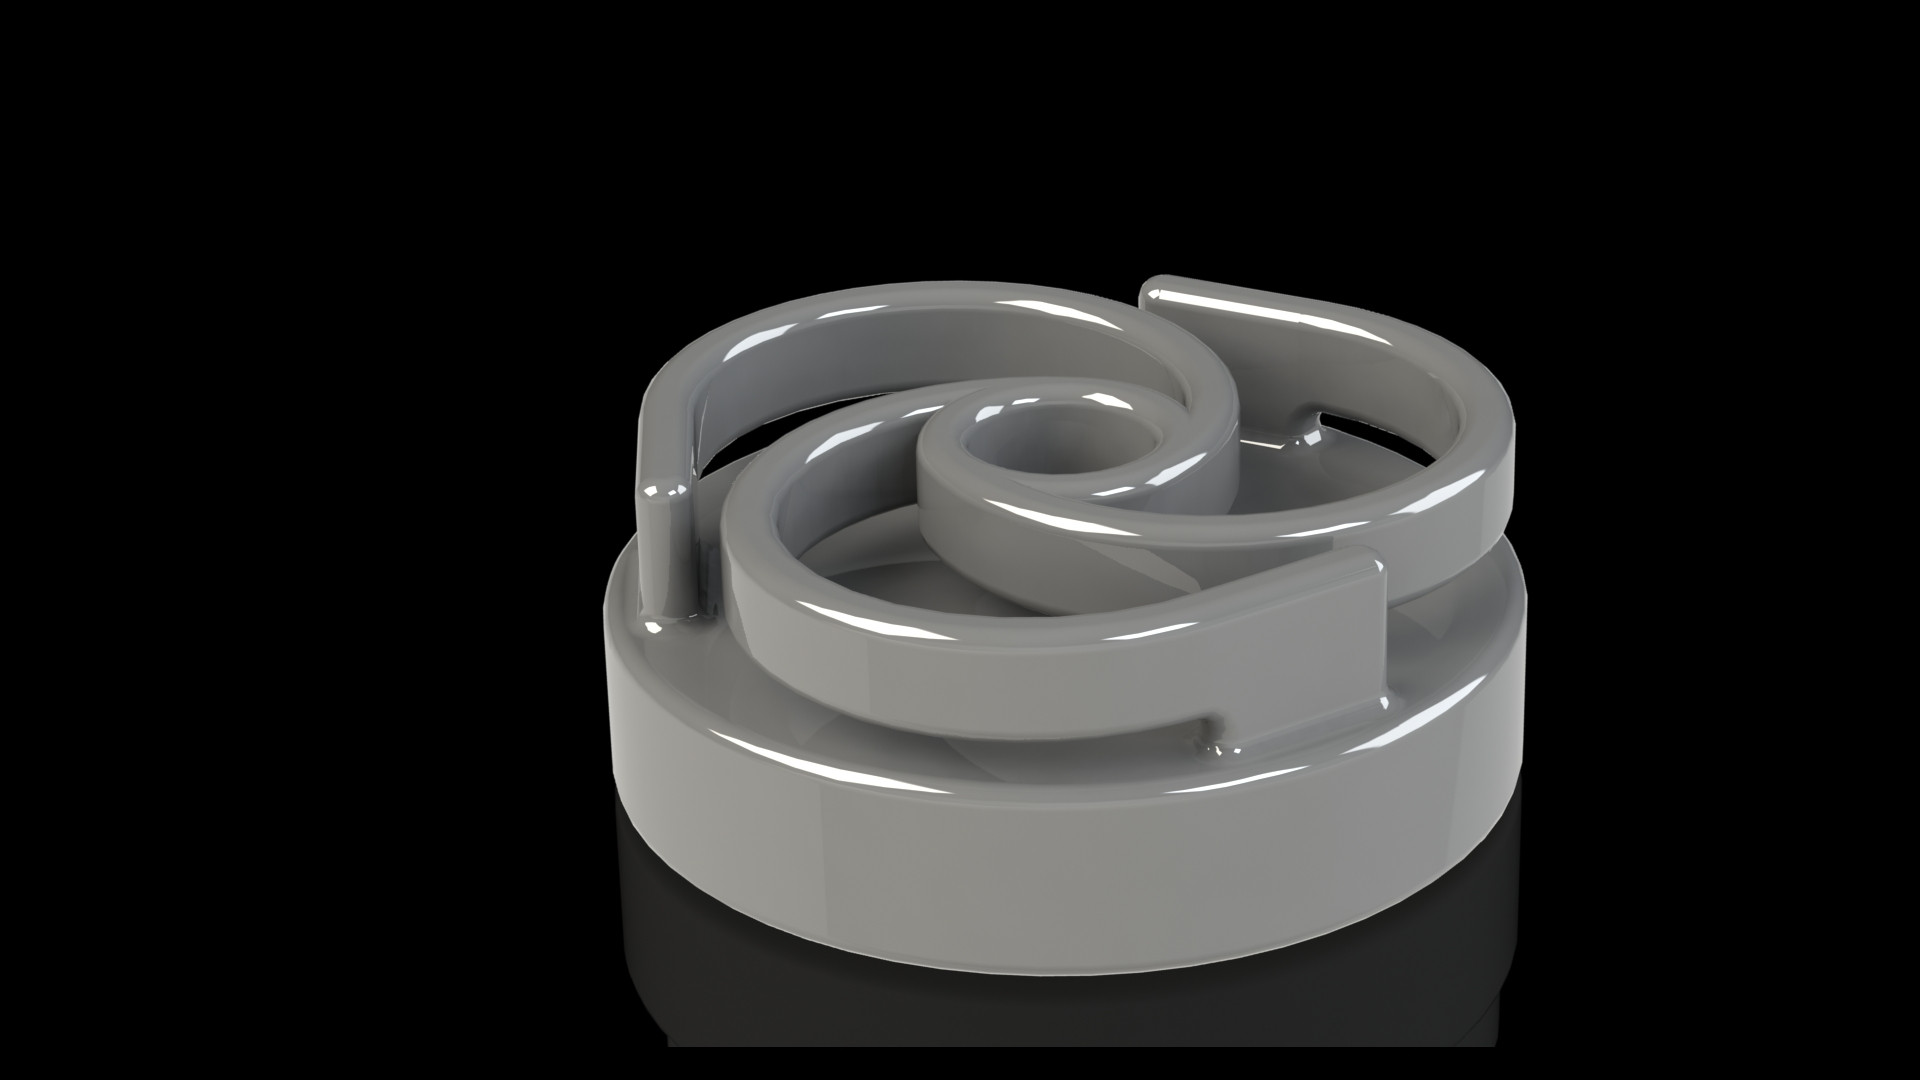
\includegraphics[width=12cm]{FlexibleCouplingRender1.JPG}
\caption{The flexible coupling for the rotary encoder}
\label{fig::FCR}
\end{figure}

The full assembly is as shown in fig \ref{fig::REA}

\begin{figure}[H]
\centering
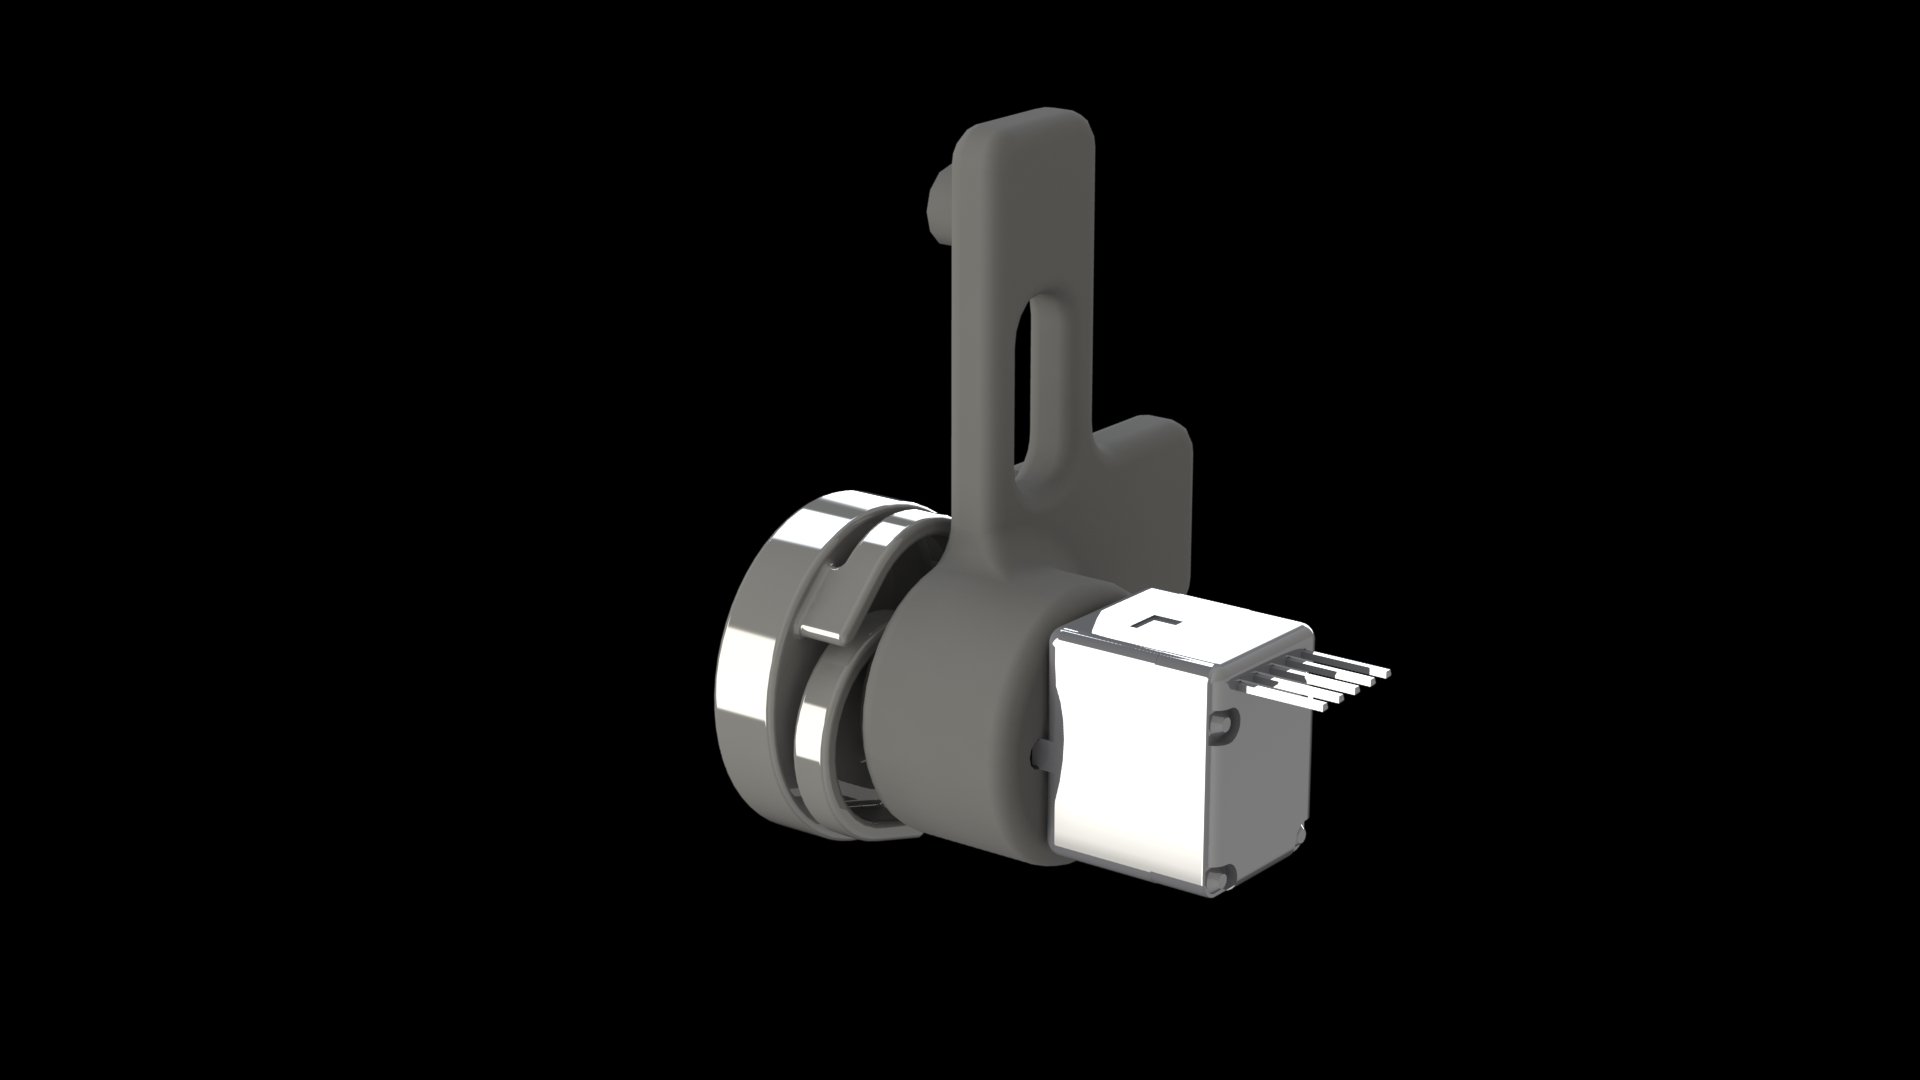
\includegraphics[width=12cm]{RotaryEncoderAssembly1.JPG}
\caption{Full assembly of the mount for the rotary encoders}
\label{fig::REA}
\end{figure}

The flexible coupling provides 5 degrees of freedom.
The coupling allows the axis to move slightly in lateral directions as relative to the axle, as well as slightly towards and away from the axle.
This has been tested in Solidworks, and a 10N force is enough to move the axle 0.5mm.

\subsubsection{Wiring}
The wiring for the encoders on the Arduino side was already in place, due to the old encoders that were since removed.
Figure \ref{fig::WD} shows the wiring.

\begin{figure}[H]
\centering
\includegraphics[width=12cm]{something.image}
\caption{The wiring of the rotary encoders}
\label{fig::WD}
\end{figure}




\section{Miscellaneous 3D Printed Parts}
For this project, extensive use was made of the 3D printer available in the innovation lab at T5.
In order to improve the presentation of WTR, as many loose parts as possible have been slotted into custom designed sleeves or boxes, clipped into place on the frame.
Some parts have been screwed into the wood, such as the 4 Raspberry Pi's, which now have increased accessibility.
Any measurements used were either looked up in the relevant data sheets, or measured using a caliper with a +-0.10mm inaccuracy.

\subsection{Boxes and Containers}
\subsubsection{IMU container}
Since the IMU needs to be away from Iron as far as possible, the decision was made to clip it to the top of the TV screen.

\begin{figure}[H]
\centering
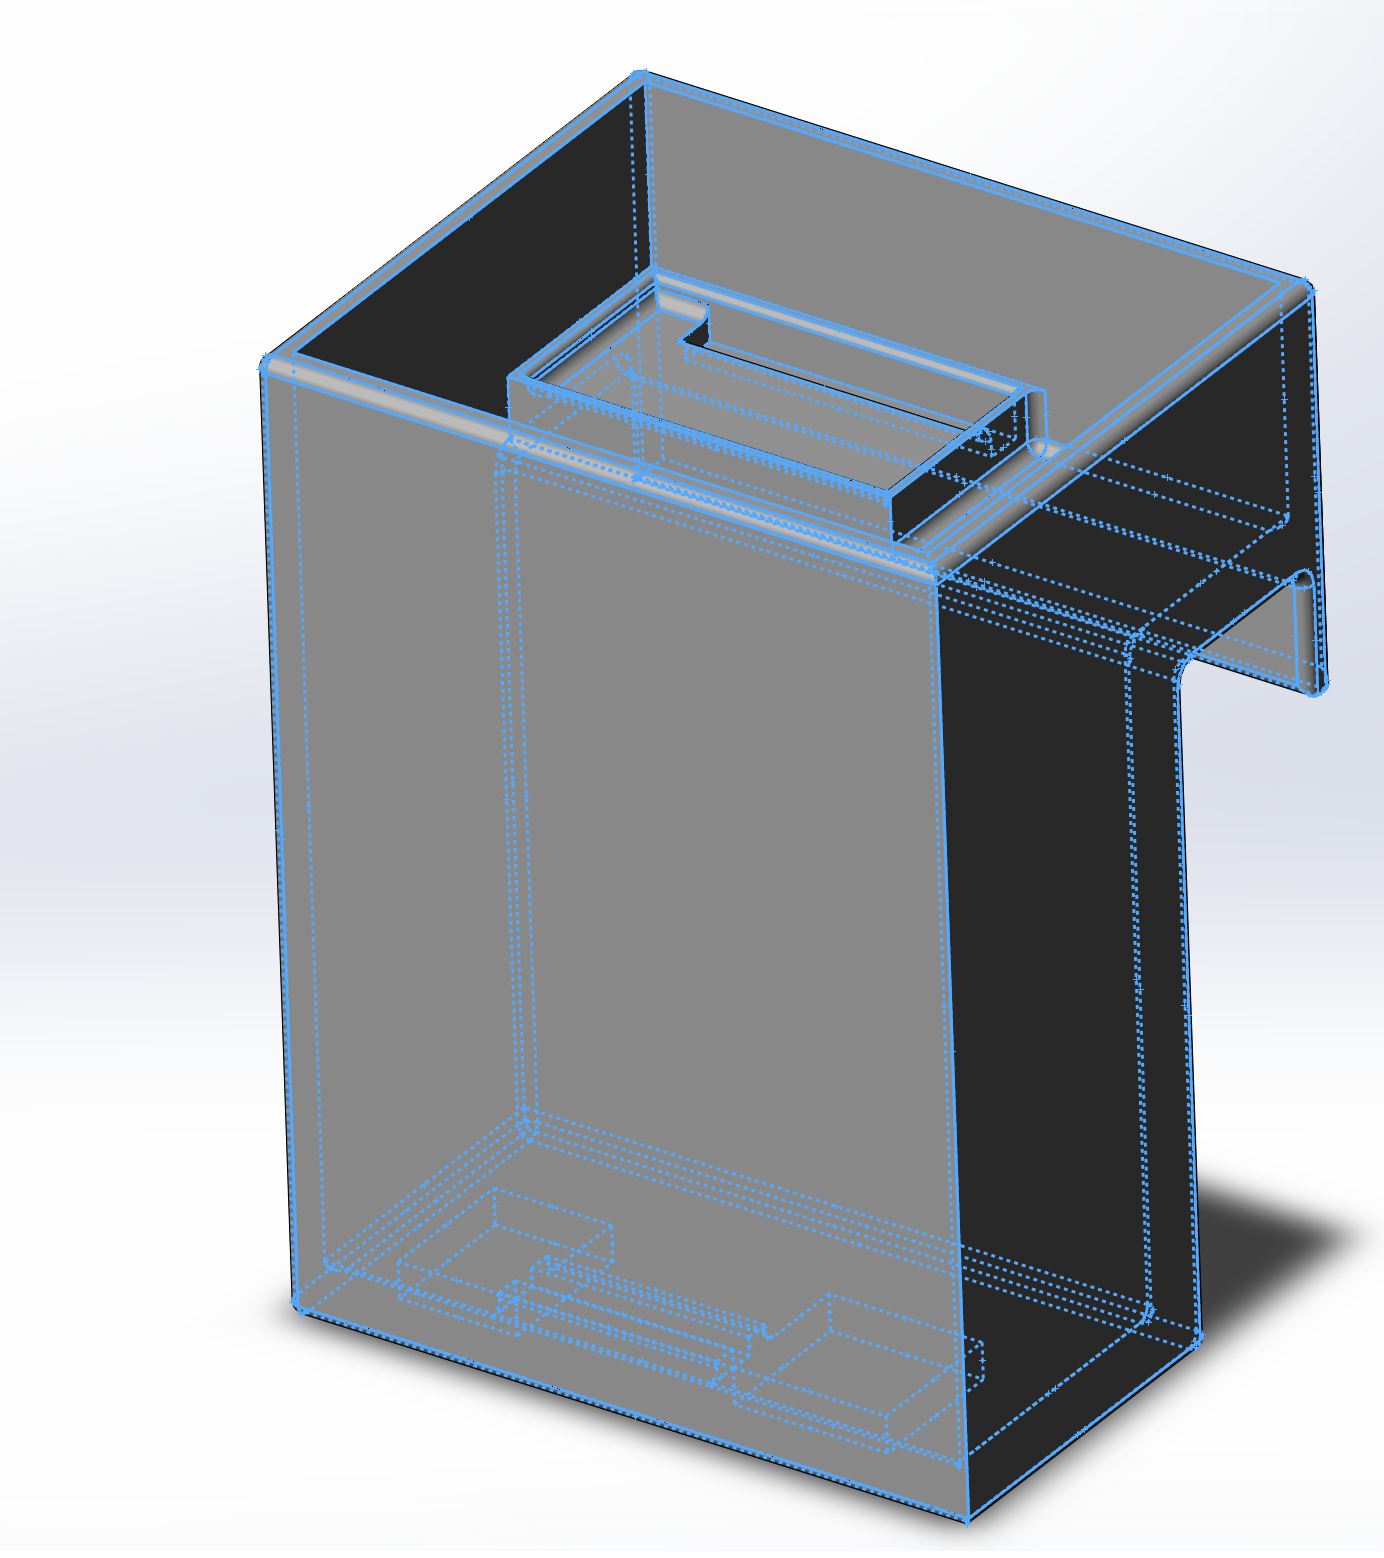
\includegraphics[width=12cm]{/3ddesign/imubak.png}
\caption{A partially wireframed model of the casing for the IMU and an Arduino}
\label{fig::IMUB}
\end{figure}

As shown in figure \ref{fig::IMUB}, the case has a hooked top, which allows it to hang to from the top of the screen.
It also has a slot for an Arduino, kept in place using the USB port, as well as the power jack.
In addition, a small slot has been made at the bottom for the PCB section to fit into.

The IMU is contained in a small rectangular section at the top, with a smaller rectangle cut out to allow the pins to slot in neatly.
A lid can be placed on top of the box, to allow it to be closed off and less likely to be interfered with.

\subsubsection{Sonar Arduino container}
The container for the arduino that pings all the HC-SR04 sensors can be found near the sensor node Pi, clipped onto the side of WTR.
It is a small box with a few rectangles cut out of the lid to allow wire to pass through, from the arduino to the sensors.

\begin{figure}[H]
\centering
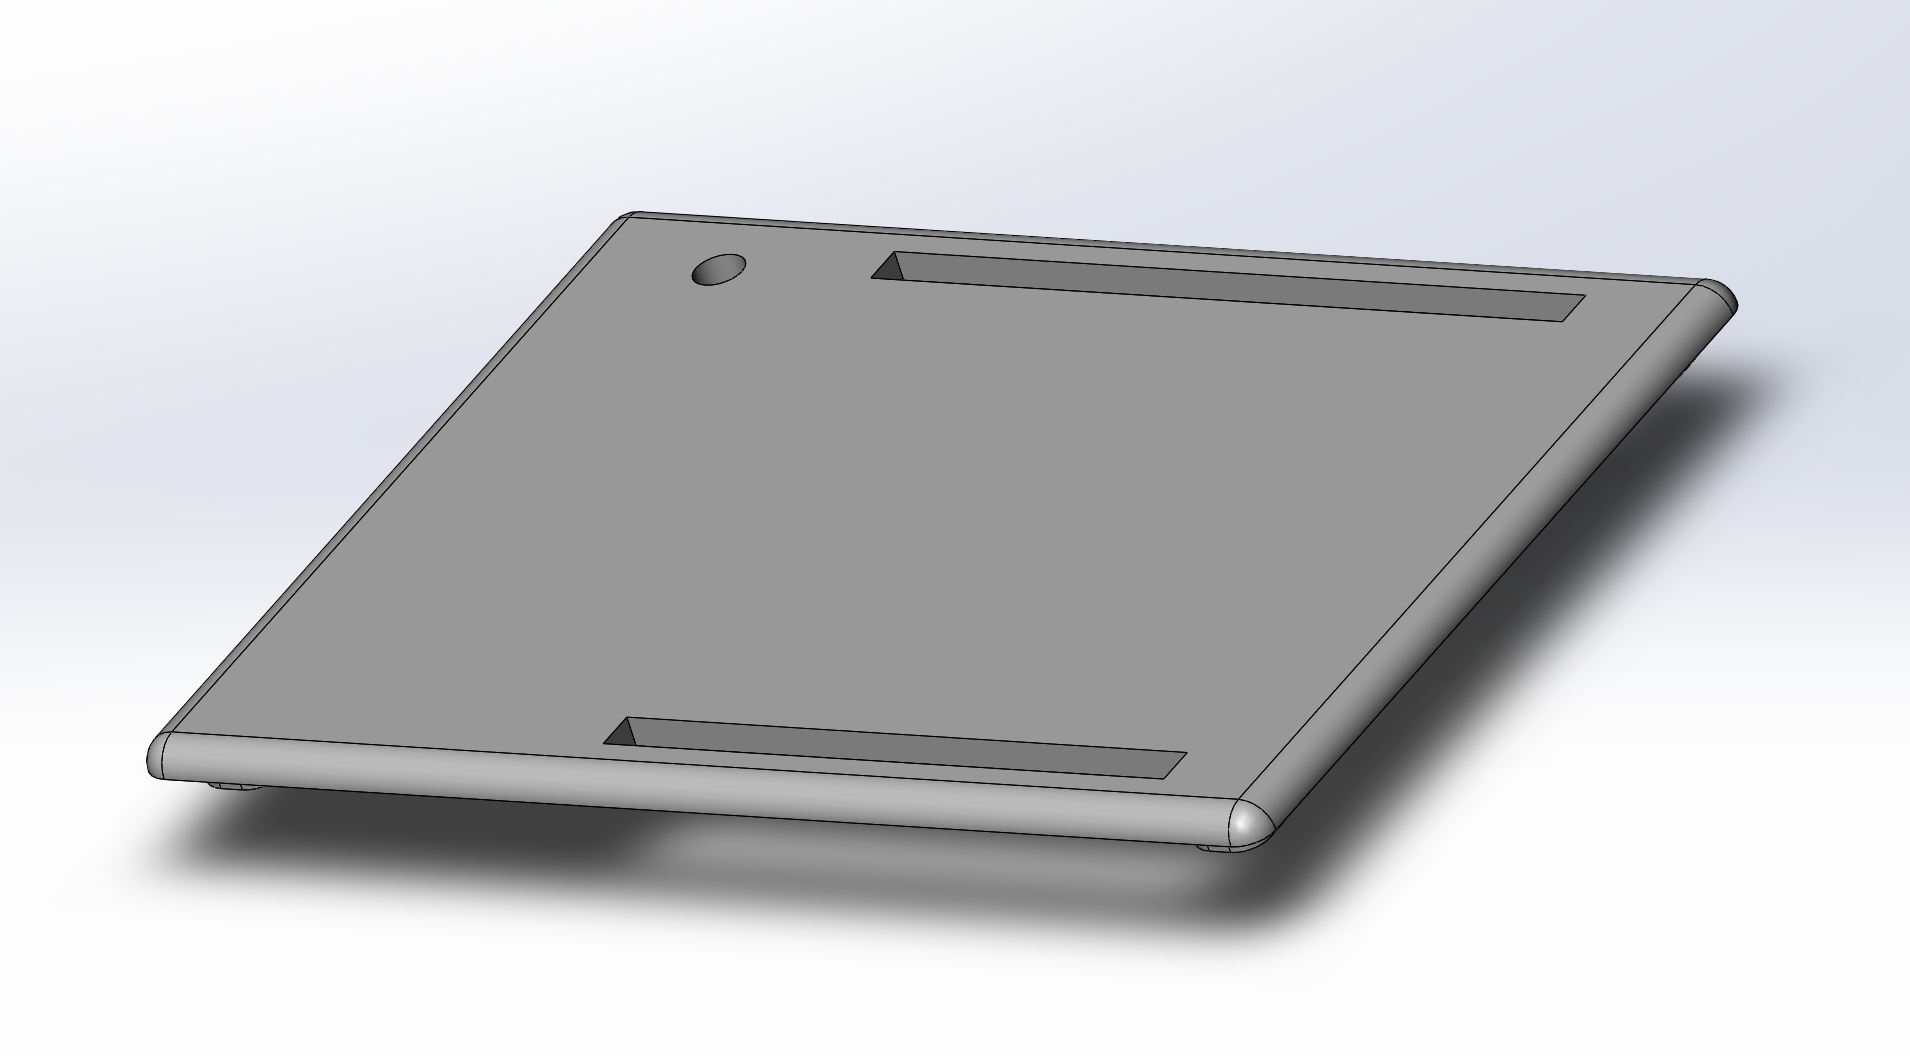
\includegraphics[width=10cm]{/3ddesign/ardlidson.png}
\caption{The lid of the arduino container}
\label{fig::ardLidSon}
\end{figure}

\begin{figure}[H]
\centering
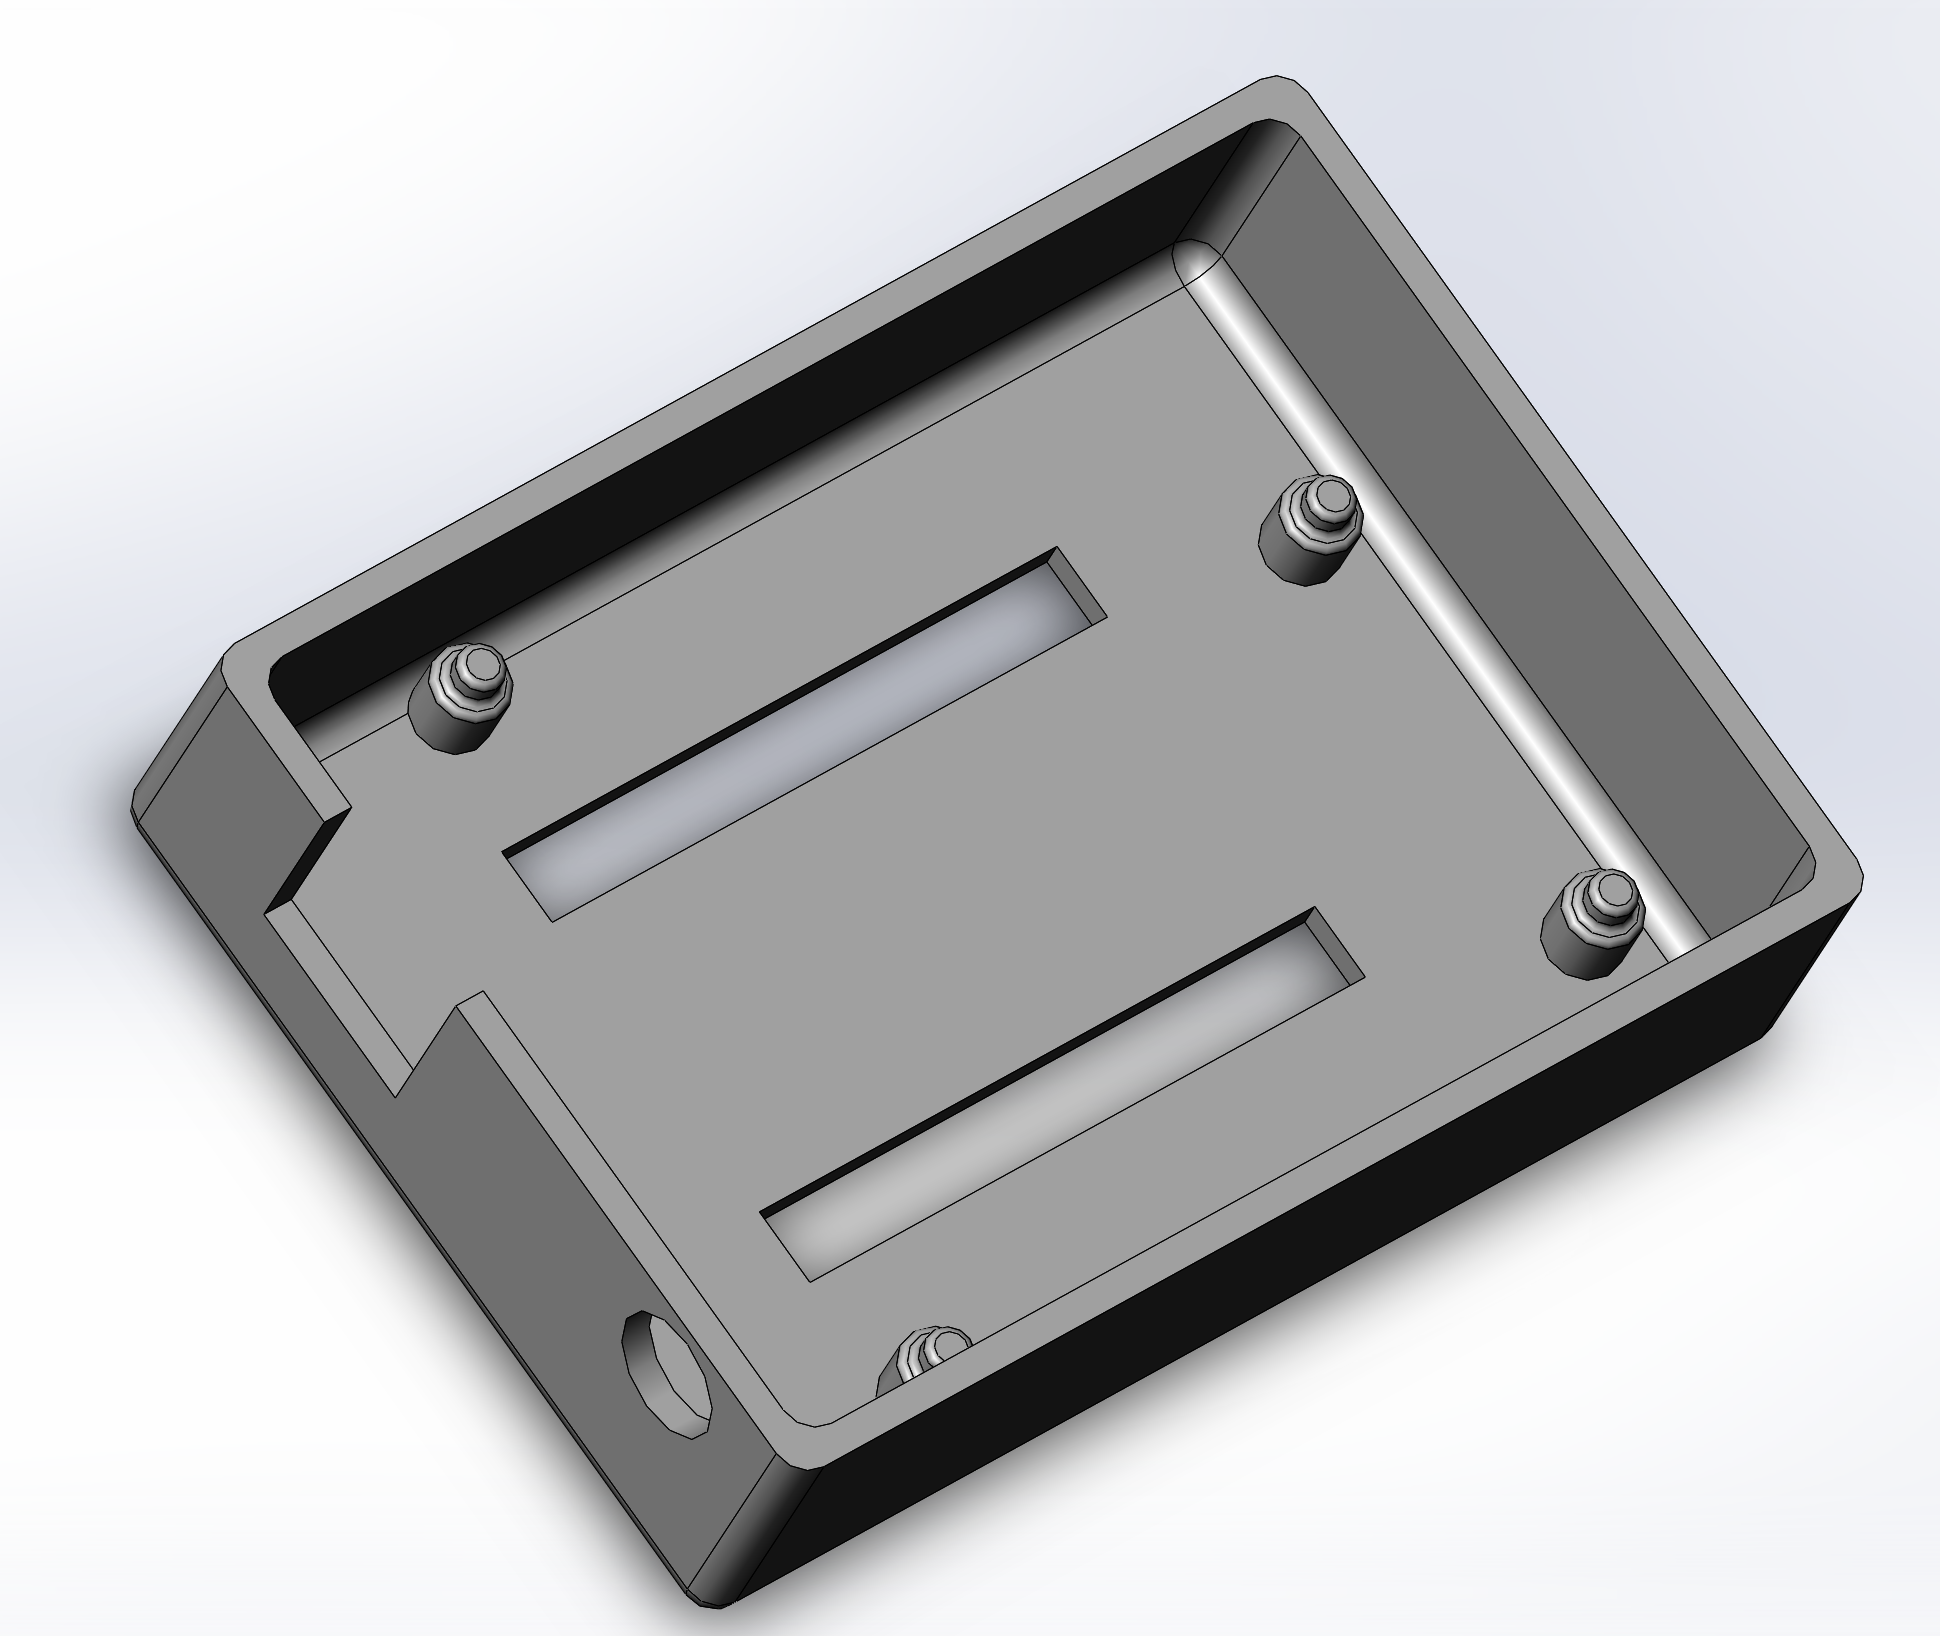
\includegraphics[width=12cm]{/3ddesign/ardconson.png}
\caption{The container of the arduino that pings the HC-SR04 sensors}
\label{fig::ardConSon}
\end{figure}

All of the arduino containers, unless otherwise specified, are attached to WTR via two slots in the bottom of the container and a clamp which fits around the metal beams the frame consists of.

\begin{figure}[H]
\centering
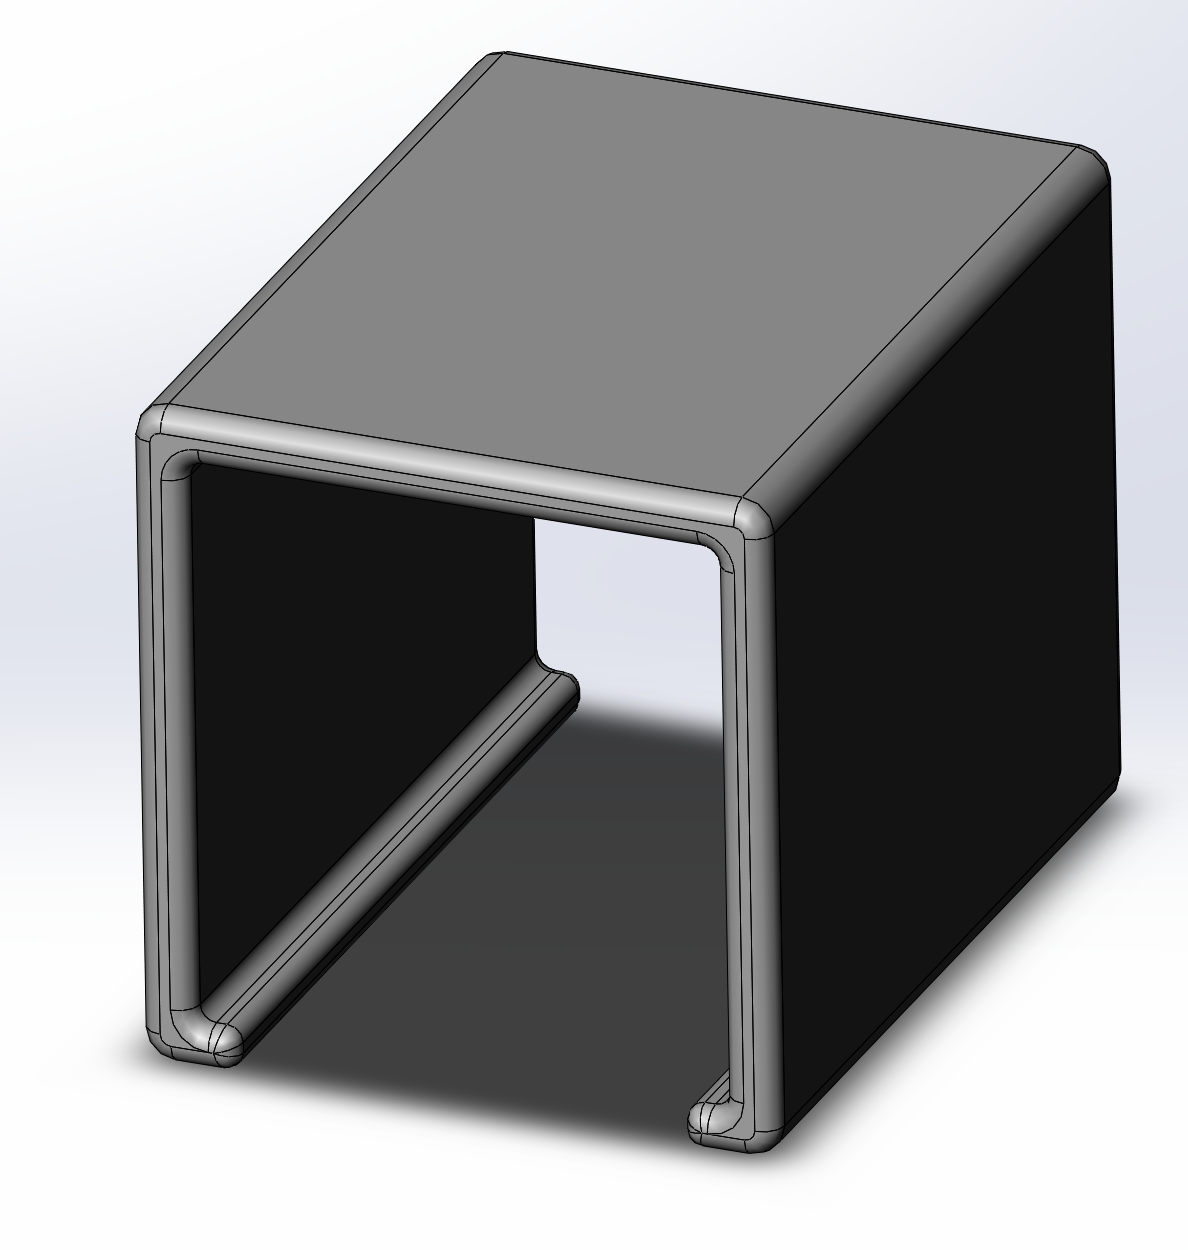
\includegraphics[width = 12cm]{/3ddesign/clamp.png}
\caption{the clamp that fits around a 25mm steel beam, with some room to spare to accommodate the containers}
\label{fig::clamp}
\end{figure}

\subsection{Emergency Stop}
The emergency stop is mounted via an open-topped box, with pins at the bottom that taper inward slightly.
This is to ensure a snug fit, which prevents the emergency stop from being removed accidentally.
Previously, it was glued to the frame via hot glue.
This is an obvious security risk, since hot glue does not adhere well to metal.

\begin{figure}[H]
\centering
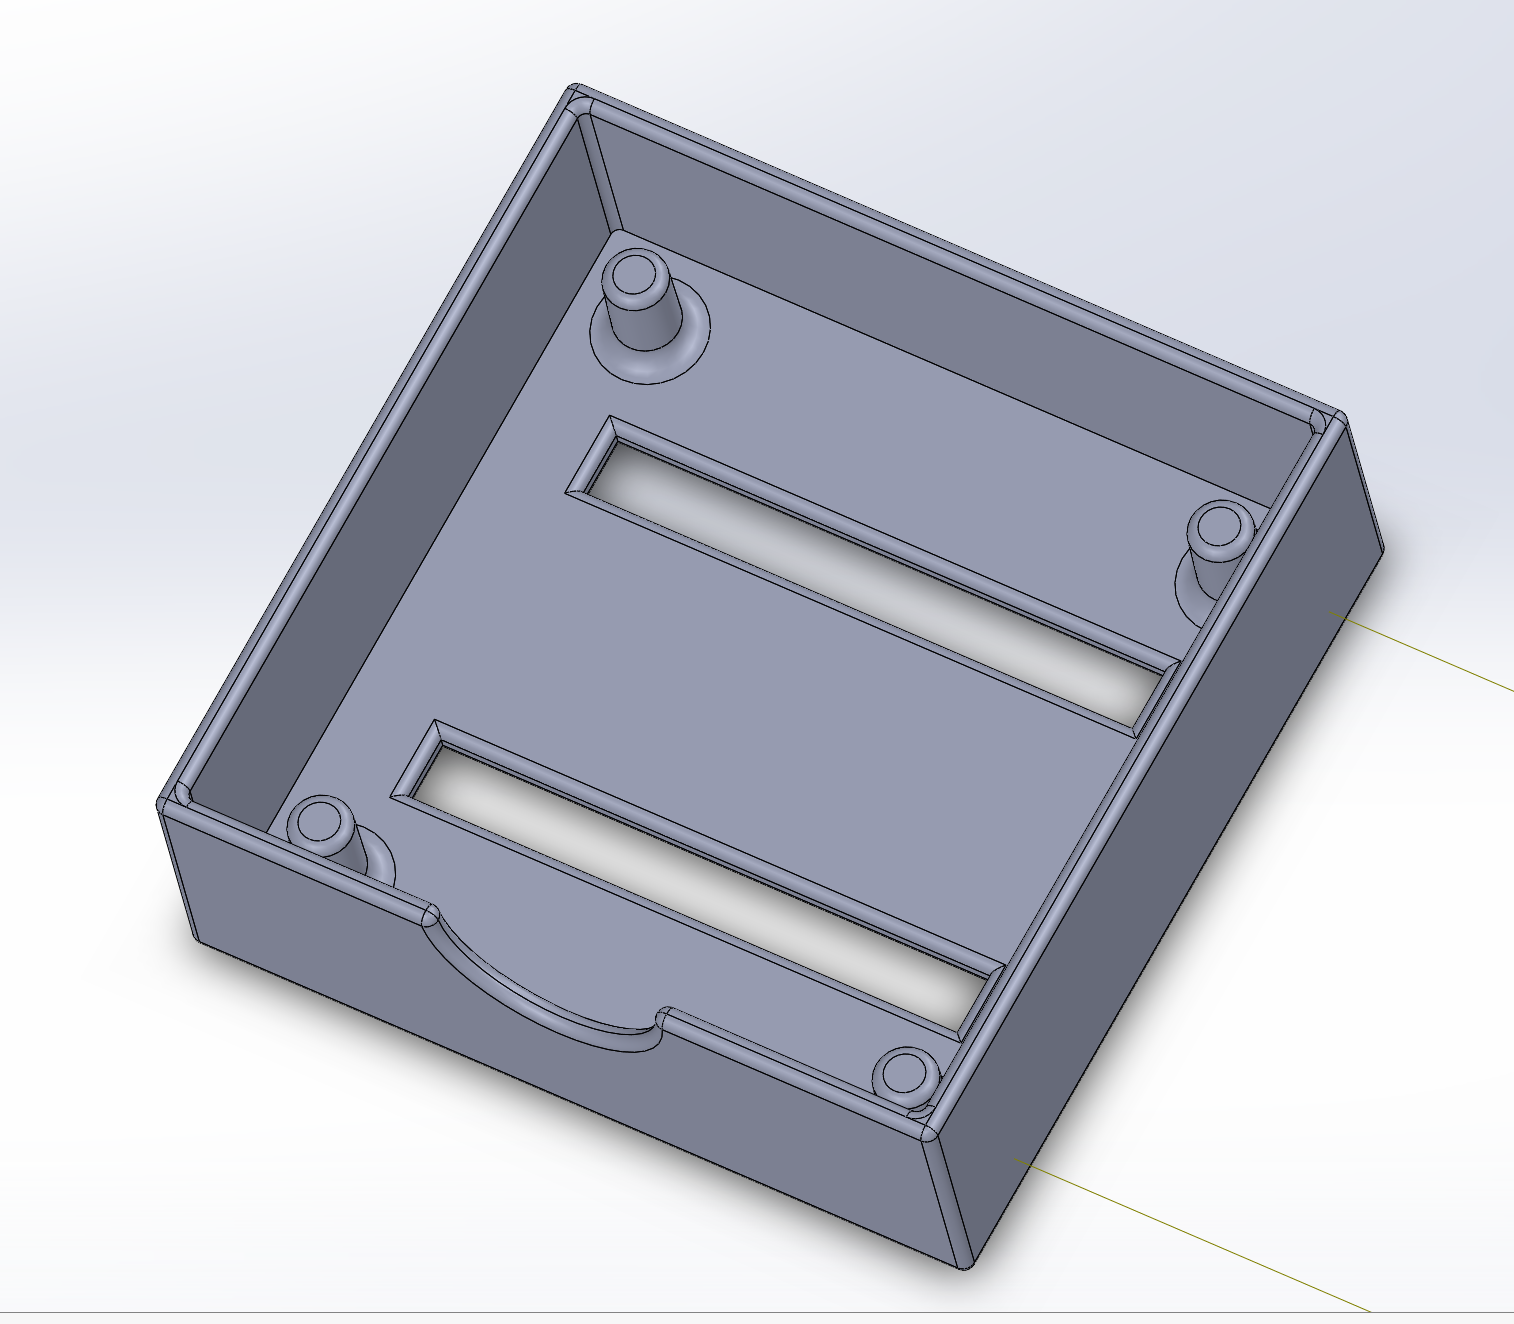
\includegraphics[width=12cm]{/3ddesign/emergency.png}
\caption{The container for the emergency stop button}
\label{fig::ESB}
\end{figure}

The container is attached to the frame using a clamp shown in figure \ref{fig::clamp}.

\subsection{PS3 Controller Hook}
The PS3 DualShock controller was previously simply left wherever space was available.
This was not presentable, and contributed to the clutter of wires.
Instead, a hook has been designed that incorporates the cable that connects the controller to the PC, and prevents it from falling off or causing clutter.

\begin{figure}[H]
\centering
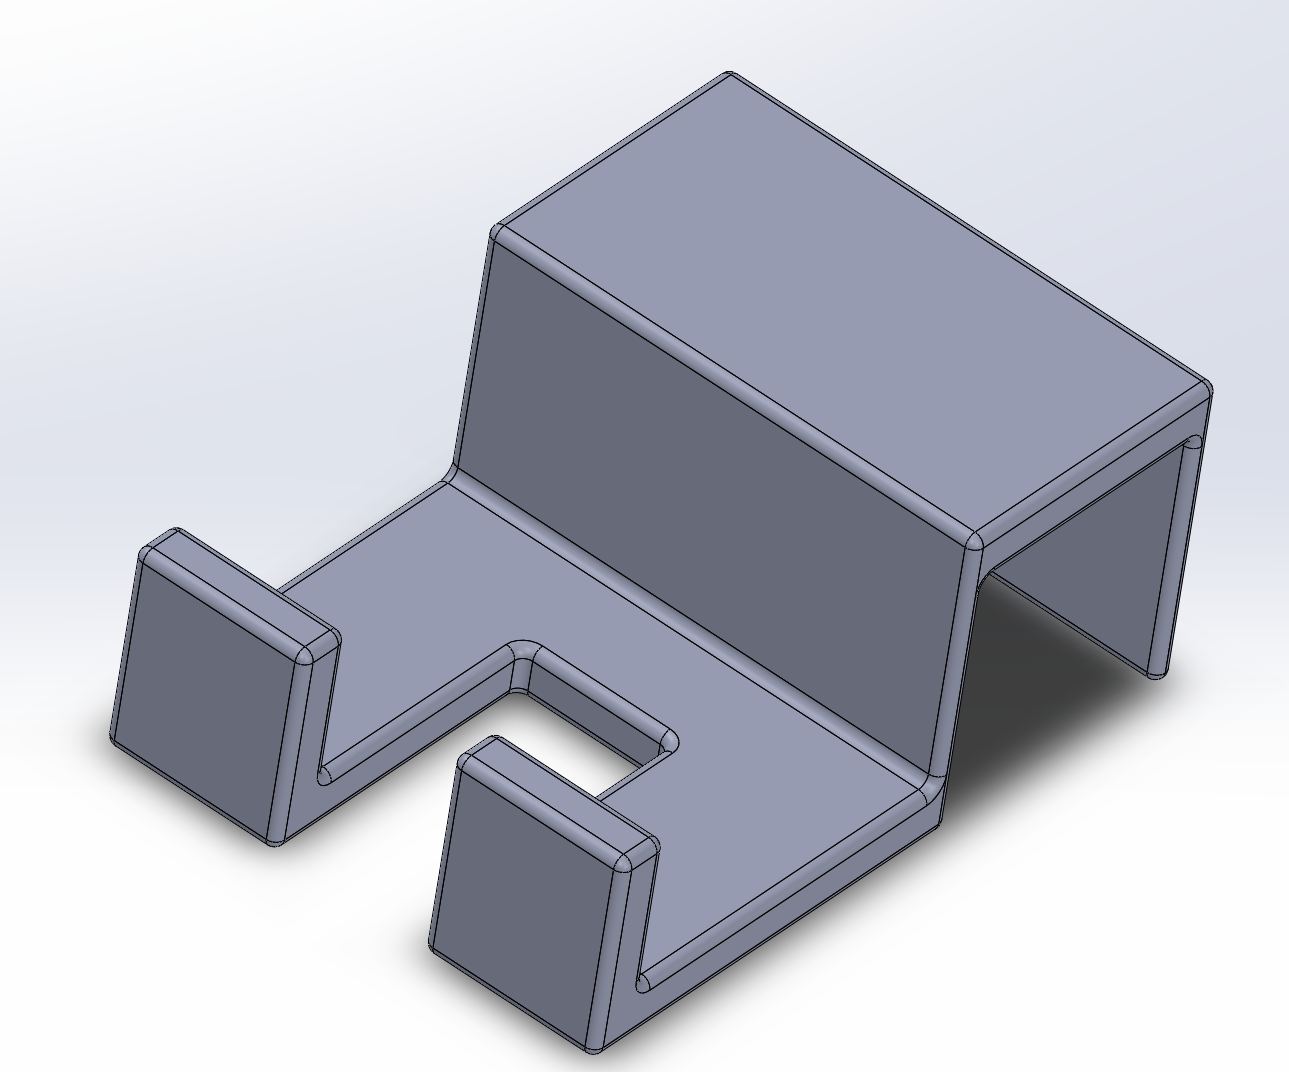
\includegraphics[width=12cm]{/3ddesign/ps3mount.png}
\caption{A mount for the PS3 controller}
\label{fig::PS3}
\end{figure}

This clamps around a metal beam much like the clamp shown in figure \ref{fig::clamp}.
It can be found above the laptop, in the middle of the frame.

\subsection{Coverings}
WTR has already claimed 2 fabric-based casualties.
2 sets of jeans have already had a hole torn in them due to sharp metal protrusions extending from the frame of WTR.
In order to prevent further incidents, some caps have been designed and printed that cover the sharp bits, without permanently removing the mounting opportunities for the white cover that can also be found in the innovation lab on T5.


\begin{figure}[H]
\centering
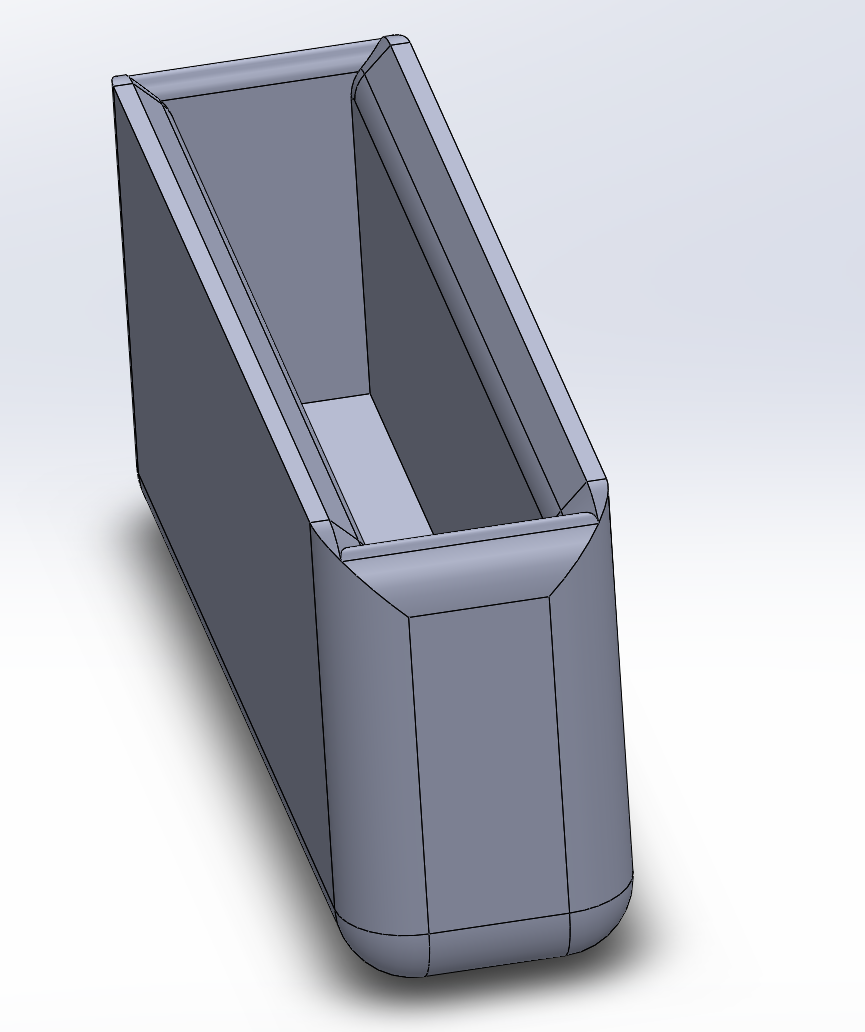
\includegraphics[width=12cm]{/3ddesign/covers.png}
\caption{The caps that cover the sharp protrusions}
\label{fig::CAP}
\end{figure}

\subsection{Fan Covering}
A cover has been designed and printed to cover the cooling fan that keeps the voltage transformers at a stable temperature.
Previously, this fan was exposed.
This is obviously a safety hazard if WTR is to be driving in public.
The cover has large enough gaps to allow airflow, but small enough to prevent accidentally touching the moving fan blades.

\begin{figure}[H]
\centering
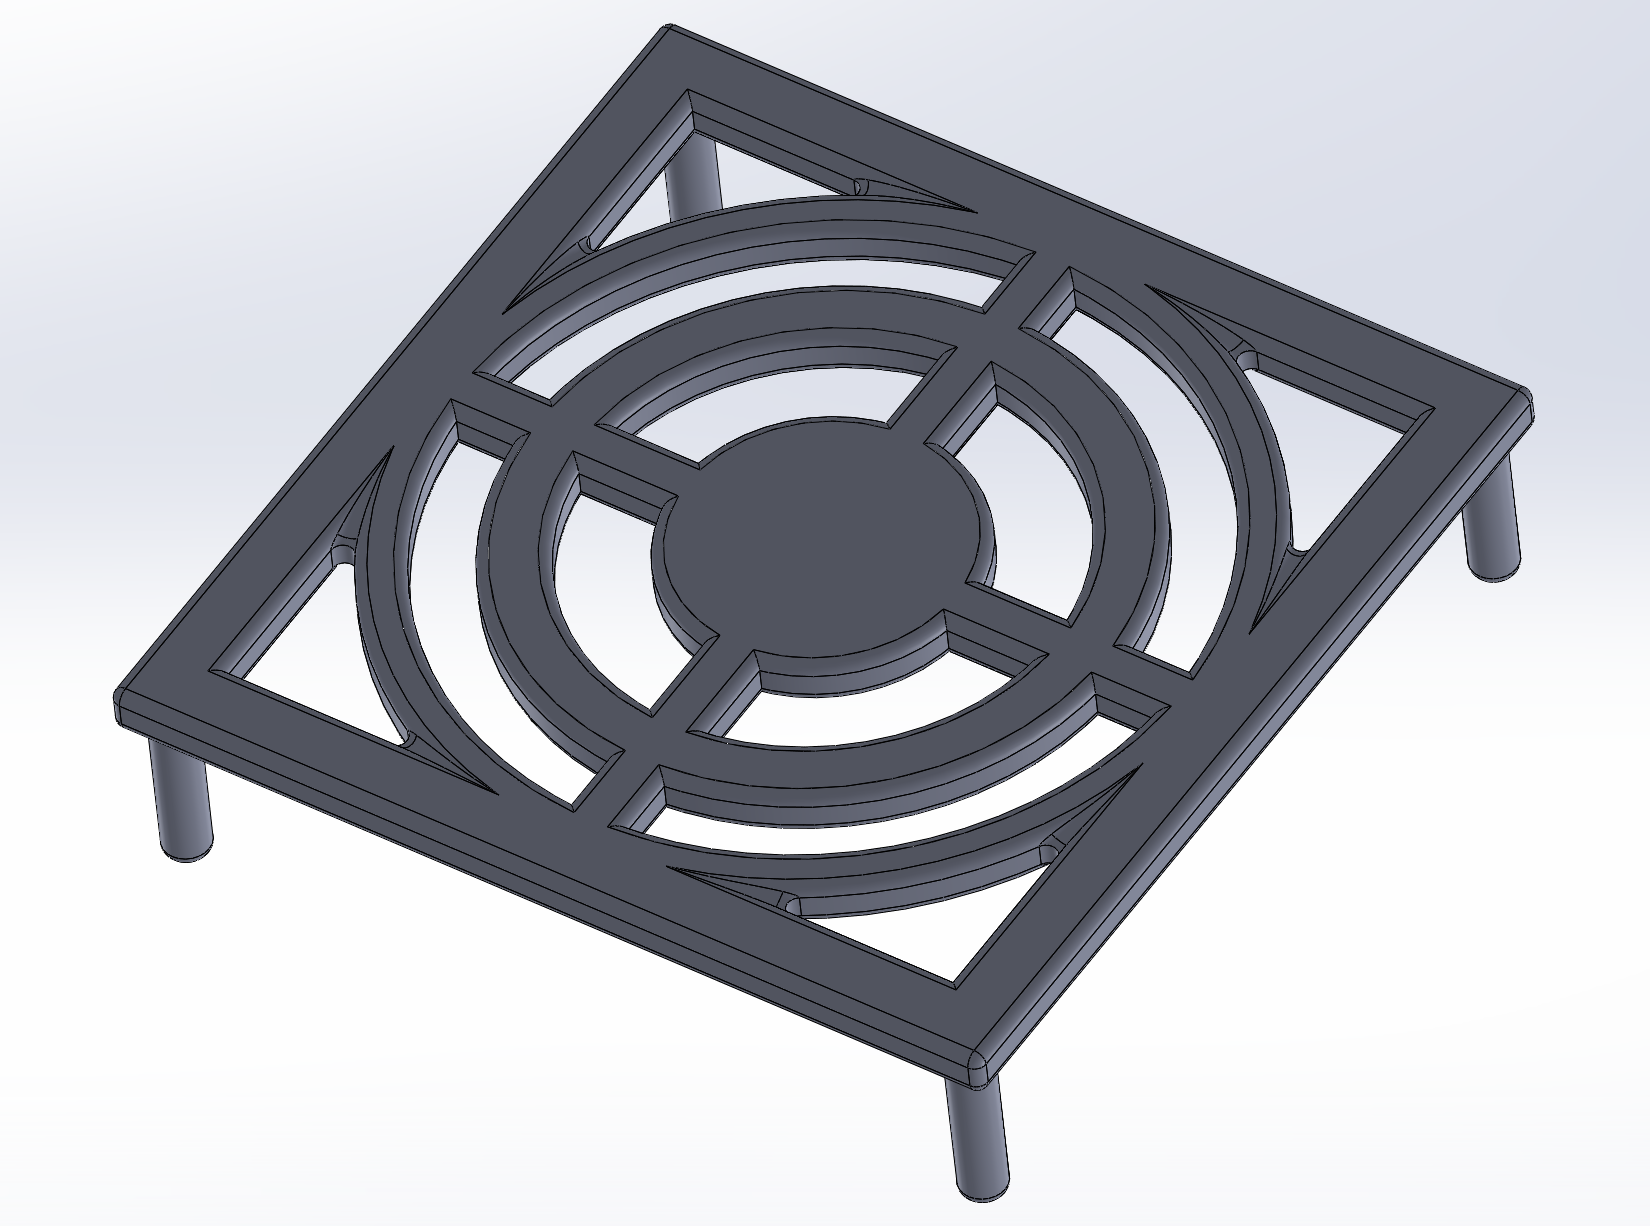
\includegraphics[width=12cm]{/3ddesign/fan.png}
\caption{A cover for the fan}
\label{fig::FAN}
\end{figure}

\subsection{Raspberry Pi Clamps}
The Raspberry Pi's used to be located in a small wooden box underneath the laptop.
They have now been moved to the front of WTR, in order to improve accessibility.
The mounts, as shown in figure \ref{fig::RPC}, have two holes in the bottom.
These fit a set of screws, and allow the mount to be attached to the wood plating.

\begin{figure}[H]
\centering
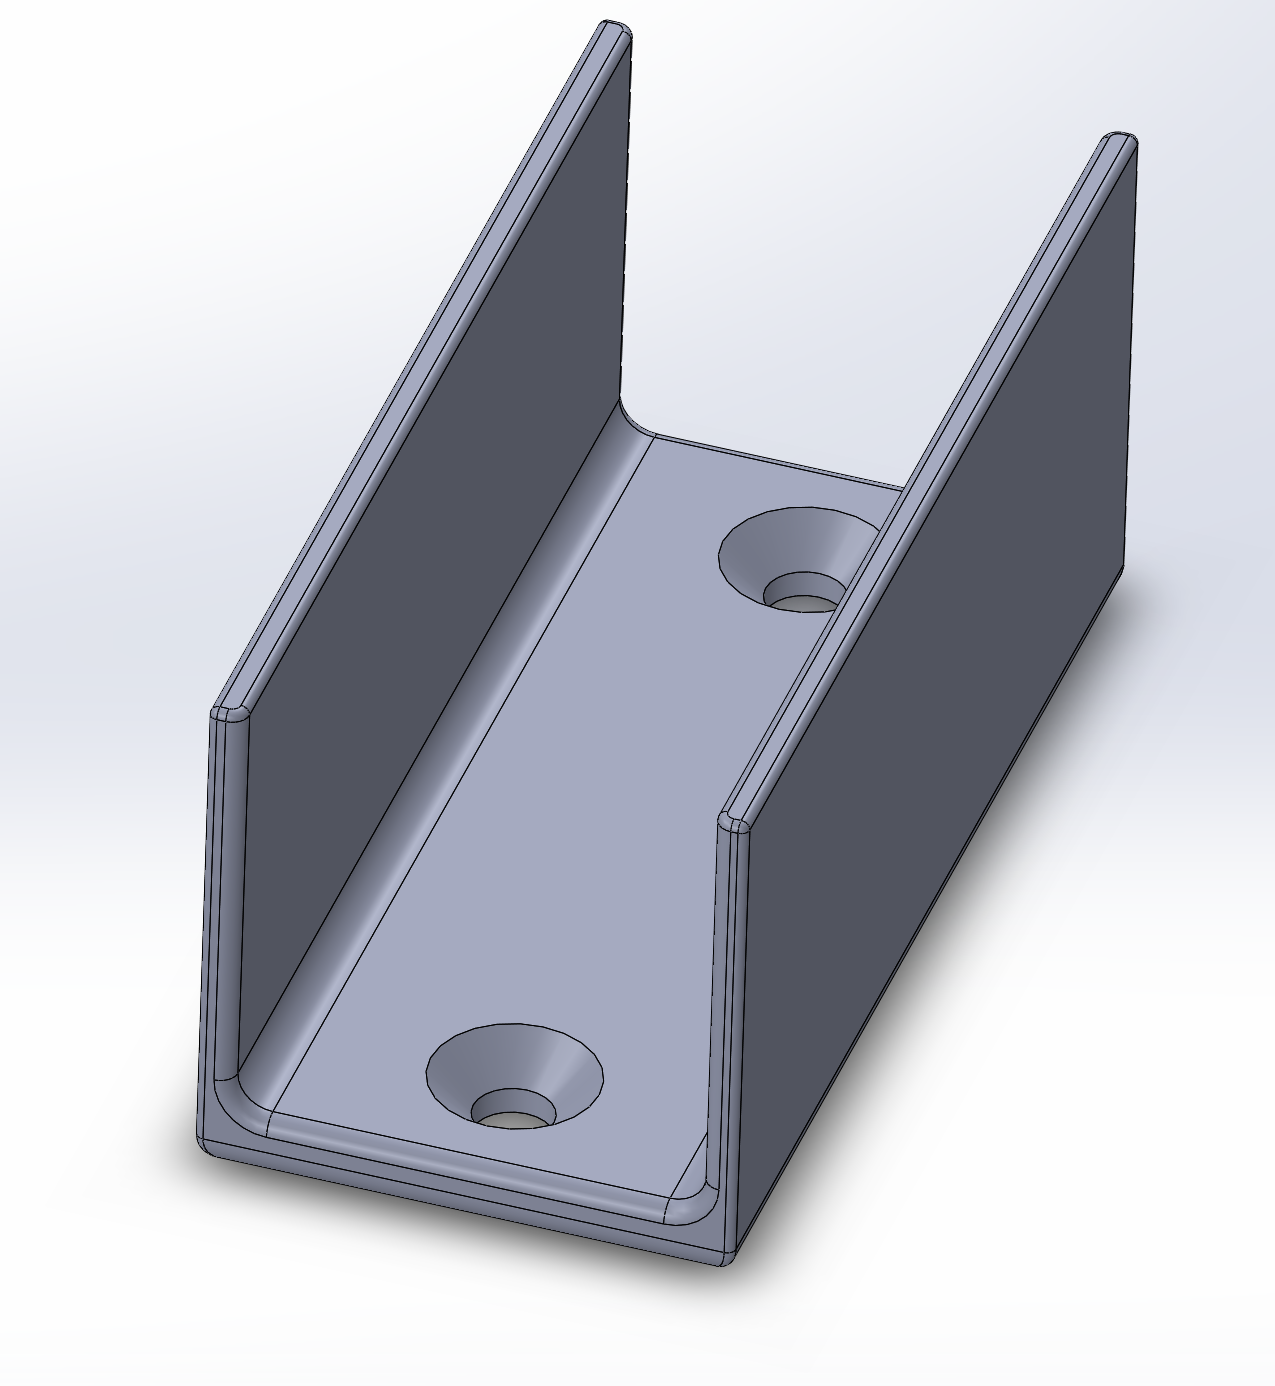
\includegraphics[width=12cm]{/3ddesign/RPC.png}
\caption{The Raspberry Pi mounts}
\label{fig::RPC}
\end{figure}


\newpage
\appendix % all sections after this are appendices
\section{Glossary}
\begin{itemize}
\item \label{trm::dms} Dead-man's switch - a button on a controlling unit which has to be held down in order to have the robot respond to inputs. This is generally done in order ensure a machine cannot perform any actions should the controller be dropped or receive inputs without proper supervision.
\item WTR - Willy The Robot.
\end{itemize}
% Bibliography:
\newpage
\bibliographystyle{apacite}
\bibliography{references}


\end{document}
